\documentclass{beamer}

\usepackage{ulem}
\usepackage[utf8]{inputenc}
\usepackage[T1]{fontenc}
\usepackage[french]{babel}
\usepackage{hyperref}
\usetheme{Warsaw} %\usetheme{CambridgeUS}


\setbeamertemplate{footline}[frame number]
\title{Uppaal, a toolbox for modelisation, simulation and verification of real time systems}
\author{Jamal \textsc{Ben Azouze}, Marien \textsc{Bourguignon}, Nicolas \textsc{De Groote}, \\Simon \textsc{Picard}, Arnaud \textsc{Rosette}, Gabriel \textsc{Ekanga}}
\date{\today}

\begin{document}

\maketitle


\begin{frame}
\frametitle{Table of Contents}
\tableofcontents
\end{frame}

\section{Introduction}
\begin{frame}
	\frametitle{Introduction}
	\begin{figure}
    	\centering
    	\includegraphics[width = 0.7\textwidth]{Uppaal.png}
  	\end{figure}
\end{frame}

\begin{frame}
	\frametitle{Features of Uppaal}
	\begin{block}{Toolbox which allows}
		\begin{enumerate}
			\item \textbf{Modelisation} of system through network of timed automata
			\item \textbf{Simulation} through a real time simulator 
			\item \textbf{Model checking} through TCTL formulas 
		\end{enumerate}
	\end{block}
\end{frame}

\begin{frame}
	\frametitle{GUI}
	\begin{figure}
    	\centering
    	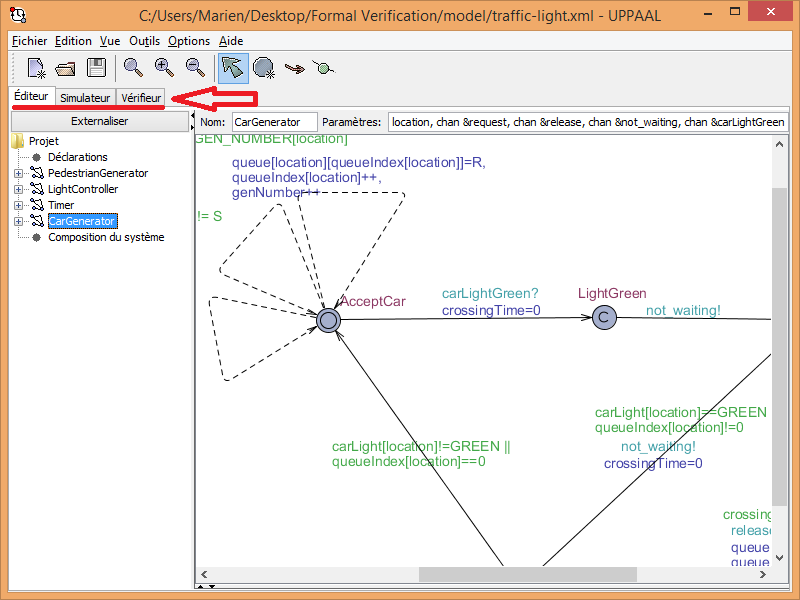
\includegraphics[width = 0.85\textwidth]{uppaal_main_window.png}
  	\end{figure}
\end{frame}

\section{Modelisation}
\begin{frame}
	\frametitle{Modelisation tool}
	\begin{block}{Model made of}
		\begin{enumerate}
			\item Extended timed automata (aka \textit{templates})
			\item Combined into a \textit{system} (network of timed automata)
		\end{enumerate}
	\end{block}
	\begin{figure}
    	\centering
    	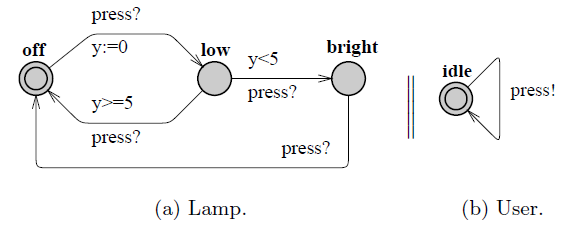
\includegraphics[width = 0.85\textwidth]{timed_automata_uppaal.png}
    	\caption{System made of ETAs. Image from \textit{A Tutorial on Uppaal}}
  	\end{figure}
	
\end{frame}

\begin{frame}
	\frametitle{Extended Timed Automata (ETA)}
	\begin{block}{Like TA, ETA are made of}
		\begin{enumerate}
			\item Vertices, called \textbf{states}
			\item Edges, called \textbf{transitions}
		\end{enumerate}
	\end{block}
	
	\begin{block}{But also}
		\begin{enumerate}
			\item Bounded integer variables
			\item Structured data types
			\item User defined functions
			\item Channel synchronization
		\end{enumerate}
	\end{block}
	
\end{frame}

\begin{frame}
	\frametitle{Back to the GUI (ft paint)}
	\begin{figure}
    	\centering
    	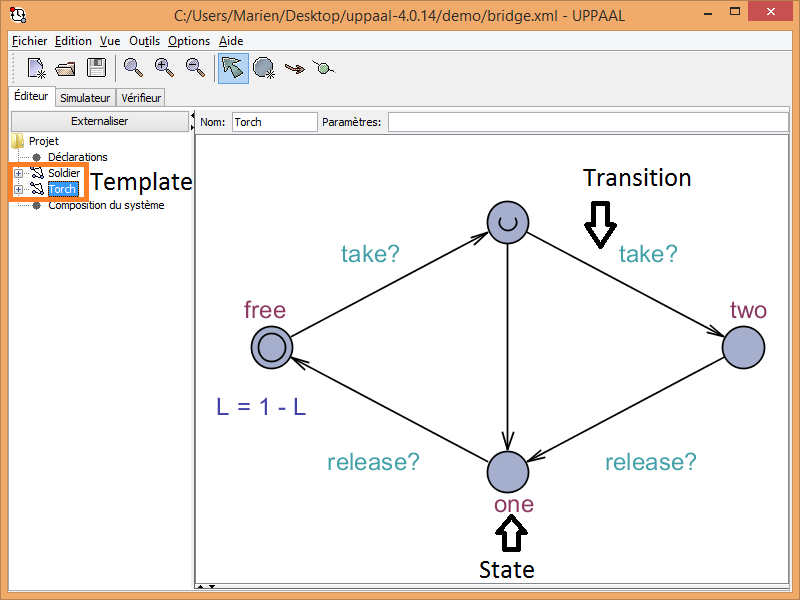
\includegraphics[width = 0.85\textwidth]{uppaal_eta.png}
  	\end{figure}
\end{frame}

\begin{frame}
	\frametitle{State (vertex)}
	\begin{figure}
    	\centering
    	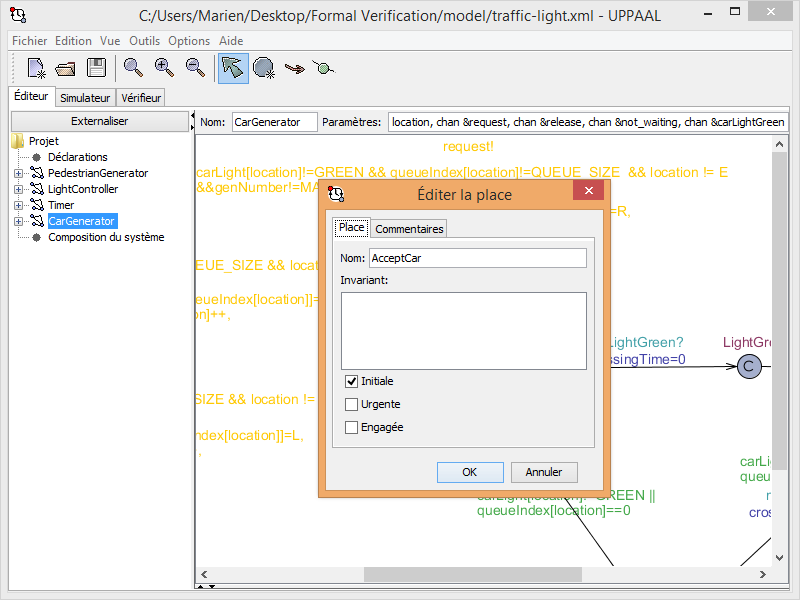
\includegraphics[width = 0.85\textwidth]{uppaal_vertex_editor.png}
  	\end{figure}
\end{frame}

\begin{frame}
	\frametitle{State (vertex) cont'd}
	\begin{block}{Edit window:}
		\begin{enumerate}
			\item \textbf{Name}: the name of the state
			\item \textbf{Invariant}: free of side effect condition, only allowed to stay if it holds
			\item \textbf{Initial state}: the initial state of the automaton
			\item \textbf{Urgent state}: Like having the following invariant x<=0 (where x is reset in the incoming transition)
			\item \textbf{Engaged state}: Like urgent (freeze time), but the next transition has to come from an urgent state
		\end{enumerate}
	\end{block}
\end{frame}

\begin{frame}
	\frametitle{Transition (edge)}
	\begin{figure}
    	\centering
    	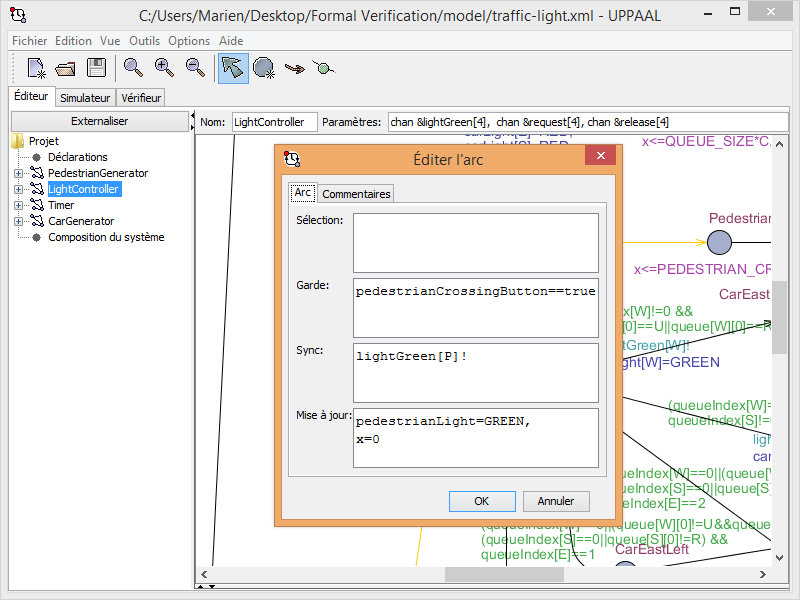
\includegraphics[width = 0.85\textwidth]{uppaal_edge_editor.png}
  	\end{figure}
\end{frame}

\begin{frame}
	\frametitle{Transition (edge) cont'd}
	\begin{block}{Edit window:}
		\begin{enumerate}
			\item \textbf{Selection}: Nondeterministically chose a value for a variable
			\item \textbf{Guard}: Invariant that has to be true to take the transition
			\item \textbf{Sync}: Either \textit{chan?} or \textit{chan!} Allow inter processes sync
			\item \textbf{Update}: Expression with side effect. Used to alter object
		\end{enumerate}
	\end{block}
\end{frame}

\begin{frame}
	\frametitle{Binary Synchronization (others are possible)}
	\begin{figure}
    	\centering
    	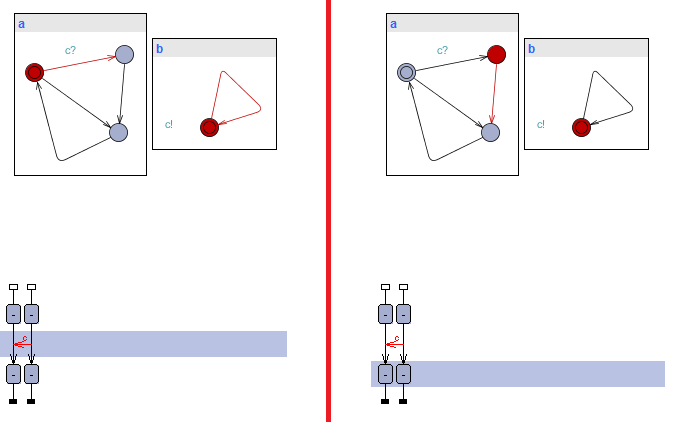
\includegraphics[width = 0.85\textwidth]{sync_before_after.png}
    	\caption{Before and after using a synchronization channel}
  	\end{figure}
\end{frame}


\begin{frame}
	\frametitle{Declaration (global or local)}
	\begin{figure}
    	\centering
    	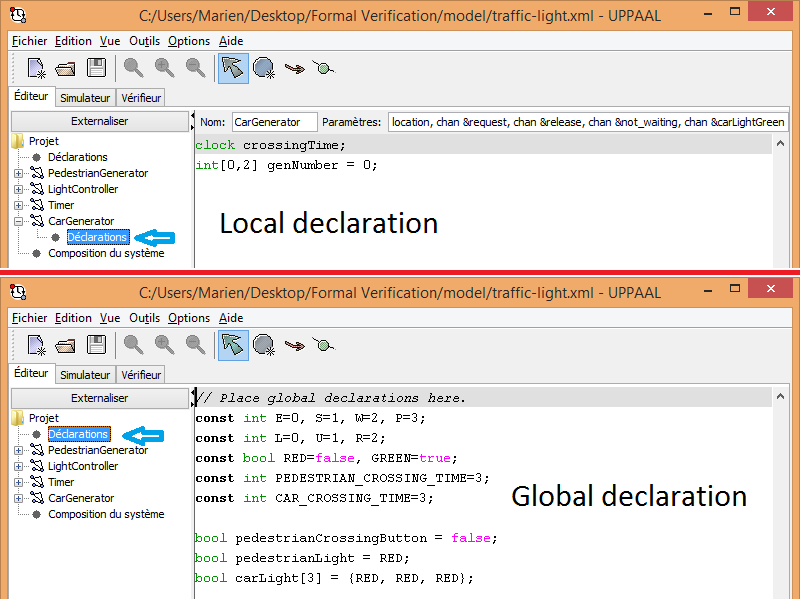
\includegraphics[width = 0.85\textwidth]{uppaal_main_window_declaration.png}
  	\end{figure}
\end{frame}

\begin{frame}
	\frametitle{Building the system}
	\begin{figure}
    	\centering
    	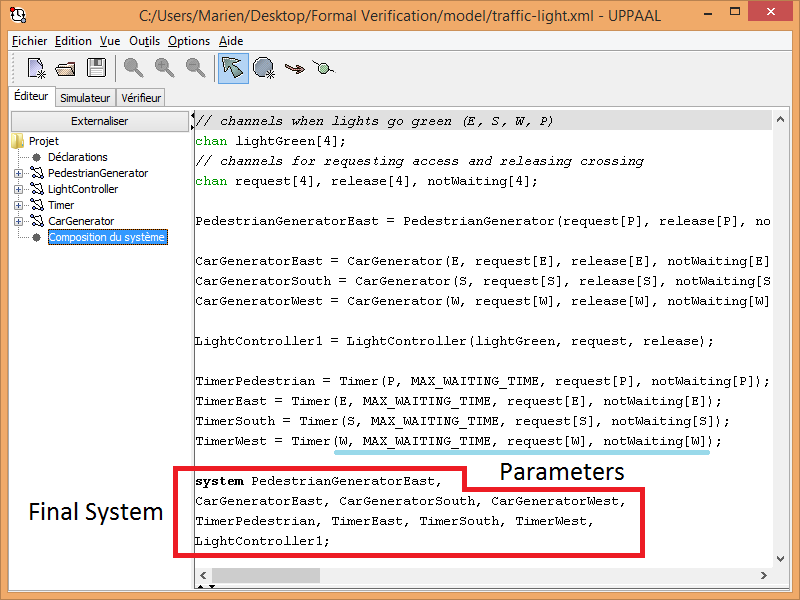
\includegraphics[width = 0.85\textwidth]{uppaal_main_window_system.png}
  	\end{figure}
\end{frame}

\section{Simulator}
\begin{frame}
	\frametitle{Features}
	\begin{block}{}
		\begin{enumerate}
			\item Manually take transitions
			\item Display the state of the system (ETA and variables)
			\item Output the trace (can be exported)
			\item Allow replay and step by step analysis
		\end{enumerate}
	\end{block}
\end{frame}

\begin{frame}
	\frametitle{GUI}
	\begin{figure}
    	\centering
    	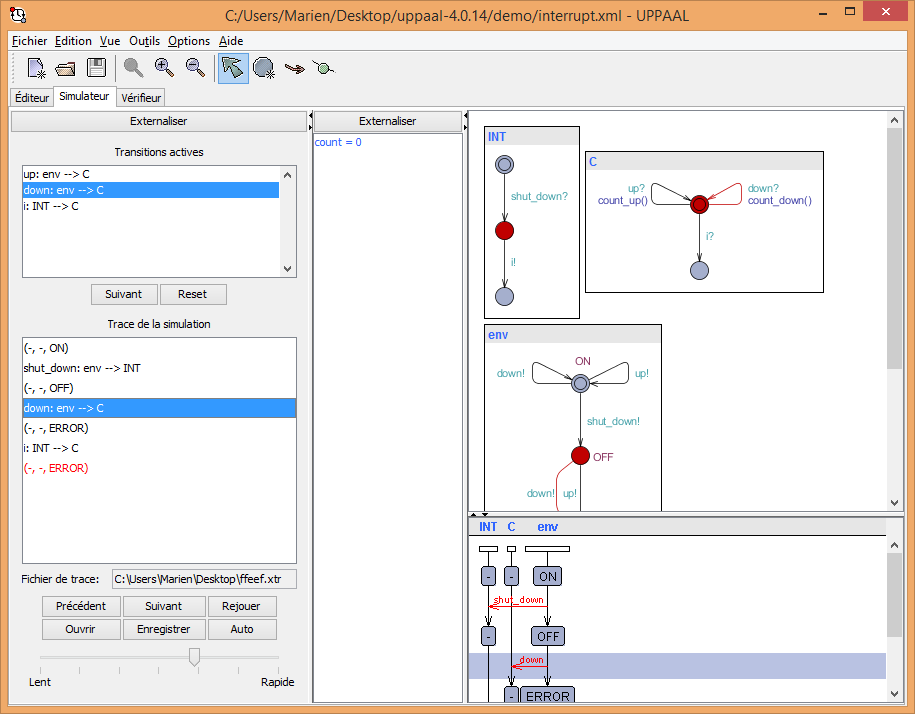
\includegraphics[width = 0.85\textwidth]{uppaal_simulator.png}
  	\end{figure}
\end{frame}


\section{Verifier}
\begin{frame}
	\frametitle{Features}
	\begin{block}{Goal}
		\begin{enumerate}
			\item Allow to verify a model according to a requirement specification
			\item Expressed formally using simplified TCTL formulas
		\end{enumerate}
	\end{block}
	
	\begin{block}{Kind of formulas}
		\begin{enumerate}
			\item State formula: describe individual states
			\item Path formula: quantify over path of the model
		\end{enumerate}
	\end{block}
	
\end{frame}

\begin{frame}
	\frametitle{Formula}
	\begin{block}{State formula}
		Expressions that are evaluated for a state, without looking at the behavior of the model
	\end{block}
	
	\begin{block}{Path formula}
		\begin{enumerate}
			\item Reachability property: can a formula be possibly satisfied?
			\item Safety property: the system never reaches a unwanted state
			\item Liveness property: the system make progress while avoiding deadlocks
		\end{enumerate}
	\end{block}
	
\end{frame}

\begin{frame}
	\frametitle{GUI}
	\begin{figure}
    	\centering
    	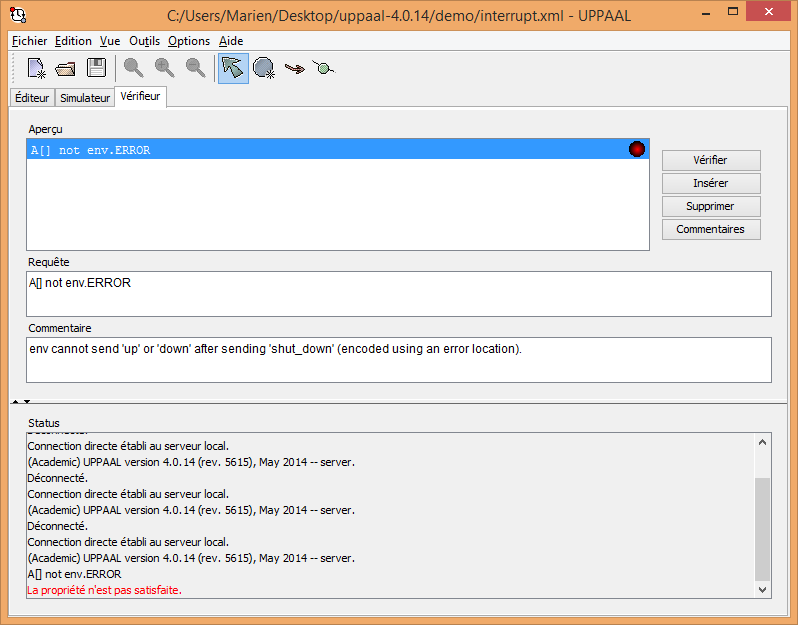
\includegraphics[width = 0.85\textwidth]{uppaal_verifier.png}
  	\end{figure}
\end{frame}

\begin{frame}[plain]
	\frametitle{Sources}
	\begin{block}{}
		\begin{itemize}
			\item \url{http://www.uppaal.org/}
			\item A Tutorial on Uppaal 4.0 - Gerd Behrmann, Alexandre David, and Kim G. Larsen
		\end{itemize}
	\end{block}
\end{frame}



\end{document}